\documentclass[11pt,letterpaper]{article}
\usepackage[margin=0.86in]{geometry}
\usepackage[T1]{fontenc}
\usepackage[utf8]{inputenc}
\usepackage{lmodern}
\usepackage{xcolor}
\usepackage{tabularx,booktabs,array,longtable}
\usepackage{enumitem}
\usepackage{hyperref}
\usepackage{fancyhdr}
\usepackage{lastpage}
\usepackage{titlesec}
\usepackage{amsmath,amssymb}
\usepackage{microtype}
\usepackage{needspace}
\usepackage{ragged2e}
\usepackage{pgfplots}
\pgfplotsset{compat=1.17}
\definecolor{navy}{HTML}{19334C}
\definecolor{teal}{HTML}{236B82}
\definecolor{soft}{HTML}{EFF5F7}
\definecolor{muted}{HTML}{52616B}
\hypersetup{colorlinks=true,linkcolor=teal,urlcolor=teal}
\titleformat{\section}{\Large\bfseries\color{navy}}{\thesection.}{0.6em}{}
\titleformat{\subsection}{\large\bfseries\color{navy}}{\thesubsection}{0.6em}{}
\titleformat{\subsubsection}{\normalsize\bfseries\color{navy}}{\thesubsubsection}{0.6em}{}
\titlespacing*{\section}{0pt}{15pt}{6pt}
\titlespacing*{\subsection}{0pt}{10pt}{4pt}
\setlength{\parindent}{0pt}
\setlength{\parskip}{4.5pt}
\setlength{\headheight}{15pt}
\renewcommand{\arraystretch}{1.16}
\setlist[itemize]{topsep=3pt,itemsep=2pt,leftmargin=1.4em}
\setlist[enumerate]{topsep=3pt,itemsep=2pt,leftmargin=1.5em}
\pagestyle{fancy}
\fancyhf{}
\fancyhead[L]{\small\color{muted} Applied Machine Learning \textbar{} Cornell Tech}
\fancyhead[R]{\small\color{muted} Human or AI?}
\fancyfoot[C]{\small\color{muted} Page \thepage\ of \pageref{LastPage}}
\renewcommand{\headrulewidth}{0.3pt}
\newcommand{\placeholder}[1]{\par\noindent\textcolor{teal}{\textit{[Your response: #1]}}\par\vspace{0.3em}}
\newcommand{\figplaceholder}[1]{\par\noindent\fcolorbox{teal}{soft}{\parbox[c][1.15in][c]{0.94\linewidth}{\centering\textcolor{muted}{Insert #1 here}}}\par}
\newcommand{\question}[2]{\needspace{4\baselineskip}\par\addvspace{0.45em}\noindent\textbf{#1}\quad #2\par\nobreak\vspace{0.1em}}
\newcommand{\smallnote}[1]{{\small\color{muted}#1}}
\newcolumntype{Y}{>{\RaggedRight\arraybackslash}X}
\begin{document}
\thispagestyle{empty}
\vspace*{0.2in}
{\color{teal}\bfseries CORNELL TECH \textbar{} APPLIED MACHINE LEARNING}\par
\vspace{0.15in}
{\Huge\bfseries\color{navy} Human or AI?}\par
\vspace{0.07in}
{\LARGE\color{navy} Kaggle Competition \&  Report Template}\par
\vspace{0.17in}

\textbf{Report Template: }\href{https://www.overleaf.com/project/6ae1fc85355dcf680137d898/share#f2777b20d3adeeecfac9096f78008e2f8daa0ff4be43de3b}{TEMPLATE}

\textbf{Github Repository Template: }\href{https://github.com/sekhari/human-or-ai-submissions}{REPO}

\textbf{Welcome to the competition!} Your task is to build a machine learning classifier that predicts whether a passage was written by a human or generated by an AI model. You will use a labeled training set, an additional unlabeled set, and a held-out Kaggle test set. The aim is not just a high leaderboard score: we want you to compare methods, design careful experiments, understand generalization, and explain what your results actually show.

You are encouraged to try several approaches. A well-tested logistic regression or support vector machine is just as legitimate as a neural network. The project is designed to be approachable on a laptop; a GPU is \emph{not required} for full credit.

\vspace{0.06in}
\begin{tabularx}{\linewidth}{@{}>{\bfseries}p{1.58in}Y@{}}
Team / members & Kexin (Cosine) Feng (kf442), Ethan Nguyen (eln39), Ketan Verma (kv293) \\
Kaggle team name & \texttt{group-number-8} \\
GitHub PR URL & \url{https://github.com/sekhari/human-or-ai-submissions/pull/20} \\
\end{tabularx}
\vspace{0.06in}
\subsection*{Your data}
\begin{tabularx}{\linewidth}{@{}lrrY@{}}
\toprule
\textbf{File} & \textbf{Rows} & \textbf{Labels} & \textbf{Purpose} \\
\midrule
\texttt{train.csv} & 10,000 & Visible & Supervised model development: 5,000 human (0), 5,000 AI (1) \\
\texttt{unlabeled.csv} & 3,000 & Hidden & Optional input for semi-supervised methods; required experiment \\
\texttt{test.csv} & 3,000 & Hidden & Predict the probability of AI authorship for Kaggle \\
\texttt{train\_starter\_2000.csv} & 2,000 & Visible & Convenient subset of \texttt{train.csv} for quick experiments \\
\bottomrule
\end{tabularx}

\smallnote{The starter data is a subset, not 2,000 additional labeled examples. Passages are approximately 75--350 words, with mean length near 210 words.}

\subsection*{How the test set works}
The test set mixes familiar and unfamiliar writing domains and AI generators, and includes some adversarially modified AI-written passages. You will \emph{not} receive labels, source model names, domain labels, or difficulty memberships for individual test examples. Submit a probability in $[0,1]$ for each test ID, where 1 means AI-generated. Kaggle evaluates submissions using \textbf{area under the ROC curve (AUROC)}. The \textbf{public leaderboard} covers 900 examples (30\%); the \textbf{private leaderboard} covers 2,100 (70\%) and determines the final competition performance score.


\vfill
\newpage
\section{Competition rubric and submission instructions}
\begin{tabularx}{\linewidth}{@{}Y>{\raggedleft\arraybackslash}p{0.85in}@{}}
\toprule \textbf{Component} & \textbf{Points}\\ \midrule
Kaggle private leaderboard performance & 25 \\
Model comparison and selection & 15 \\
Effect of training data size & 10 \\
Learning from unlabeled data & 5 \\
Generalization and error analysis & 20 \\
Open-ended improvements and insights & 15 \\
Code submission and GitHub PR history & 10 \\
\midrule \textbf{Total} & \textbf{100} \\ \bottomrule
\end{tabularx}

\textbf{How to use this document.} Complete the response fields and tables below; insert plots where requested. Keep your answers concise, specific, and supported by actual experiments. Points appear in brackets beside each question; no separate writing-quality grade is assigned.

\textbf{How credit is awarded.} We grade the \emph{quality of the experimental method, evidence, and interpretation}, not whether a proposed idea succeeds. \textbf{Negative results can also earn full credit} when the comparison is valid, the results are reported accurately, and the conclusions are thoughtful. For each question, make clear what you tried, what you measured, and what you learned. Do not invent scores or results.

\textbf{Submit three items:} (1) final Kaggle submission; (2) this completed report as PDF; (3) one GitHub PR link in the course repository, with runnable code, instructions and meaningful commit history. Include the PR link on the title page. Confirm upload locations and deadline time on the course site. The template for the repository is \href{https://github.com/sekhari/human-or-ai-submissions}{here}

\textbf{Compute and models.} Use models and pipelines that you can run and reproduce. Laptop-friendly training is strongly recommended; use of more expensive methods is allowed but not required for full credit. Do not use external LLM APIs to directly label or predict the competition test passages. Use only the supplied labeled dataset for supervised labels; allowed pretrained weights and AI-assisted development should be disclosed.

\textbf{Validation.} For the required controlled experiments, reserve a fixed stratified \textbf{2,000-row validation set} from \texttt{train.csv}, leaving up to 8,000 rows for training. Use the \emph{same} held-out validation set for comparisons and do not tune on test labels. You may retrain your final Kaggle model on all 10,000 labeled examples after selecting your approach. Where possible, document seeds and avoid source/near-duplicate leakage.

\textbf{Kaggle grading (25 points).} Final performance will use the private AUROC, not leaderboard rank. The intended continuous rule is $25\,\mathrm{clip}((A-0.50)/(T-0.50),0,1)$, where $A$ is your private AUROC and $T$ is the announced full-credit threshold. A provisional value of $T=0.90$ is under consideration; the instructors will confirm the fixed threshold before launch. A reference word TF-IDF and logistic regression baseline achieves approximately 0.868 private AUROC.

\section{Team information and model summary}
\question{Q0.1 [0 points].}{List team members and their main contributions.}

Kexin (Cosine) Feng (kf442), Ethan Nguyen (eln39), and Ketan Verma (kv293). Most of the work was done together in person. We discussed the models together, read the AI assistant's answers together, and met at least four times. Came up with the stratagy together, validate the code together, submitted the code on Cosine's laptop each time after our discussion. The modeling in this report is that shared work on \texttt{lr\_bpe}, \texttt{sgd\_bpe}, \texttt{gbm\_format}, \texttt{ENS\_top2}, and \texttt{ENS\_top3}.

\question{Q0.2 [0 points].}{Summarize your final approach in 3--5 sentences. What is the overall pipeline from raw text to probability?}

We reserve a stratified 2{,}000-row validation set from \texttt{train.csv} with seed 20261023 (1{,}000 human and 1{,}000 AI; no shared ids and no identical strings). Two models score each passage. The wording model flattens whitespace, tokenizes with a byte-level BPE model trained from scratch (vocabulary 30{,}000), and fits an SGD classifier on TF-IDF of token 1--3 grams. The layout model never reads the words: it builds 21 formatting features from the raw string and fits a histogram gradient booster. The submitted value is the equal-weight average of the two models' percentile ranks on the file being scored. For Kaggle we refit both classifiers on all 10{,}000 labels. Every validation number below instead fits only on the 8{,}000-row partition, with the locked settings in \texttt{pipeline/config.py}.

\question{Q0.3 [0 points].}{Record your final scores (enter private score only once it is revealed).}
\begin{tabularx}{\linewidth}{@{}Yp{1.8in}@{}}\toprule Metric & Your score \\ \midrule
Validation AUROC & 0.9978 \\
Kaggle public AUROC & 0.95611 \\
Kaggle private AUROC & not yet revealed \\
\bottomrule\end{tabularx}

\smallnote{Validation AUROC is \texttt{ENS\_top2} on the fixed 2{,}000-row holdout. It is not a leaderboard score. The public score 0.95611 is the Kaggle score of the uploaded submission. The private score is not yet revealed. The same collection is on both sides of the validation split, and several strong layout cues may be artifacts of how the files were saved, so the private test can be harder.}

\newpage
\section{Model comparison and selection (15 points)}
\textbf{Learning goal:} demonstrate sensible representation choices, comparisons of at least three approaches, appropriate hyperparameter selection, and evidence-based selection of the final classifier.

\question{Q1.1 [3 points].}{How did you preprocess and represent the text? Specify tokenization, normalization, word/character features or embeddings, and any feature extraction choices. Why?}

We keep two views of each passage, and we do not stem, lemmatize, or drop stop words. For the wording view we collapse every whitespace run to a single space, then train a byte-level BPE tokenizer from scratch on the fitting documents only (vocabulary 30{,}000, minimum frequency 2, no pretrained weights). Case is left as written. A TF-IDF vectorizer then takes token 1--3 grams with sublinear term frequency, minimum document frequency 2, and at most 500{,}000 features. On the 8{,}000-row partition that matrix has 389{,}838 columns. Subword grams still fire when a generator prefers a distinctive phrase, and sublinear TF keeps a long page from dominating by raw count.

The layout view is 21 counts on the raw string, mostly per 100 words or per line: blank lines, newlines, mid-sentence line breaks, line-length mean and standard deviation, markdown bullets, numbered lines, headings and bold, quotation marks, how the passage starts and ends, non-ASCII characters, curly quotes, and em dashes. On the training partition, a blank line appears in 0.4\% of human passages and 66.3\% of AI passages, while mid-sentence newlines are common in human text (1.58 per 100 words) and rare in AI text (0.014). Those cues are strong inside this collection. They can also be an artifact of saving the files, which is why the submission keeps a wording model beside them.

\question{Q1.2 [5 points].}{Which \textbf{three or more} modeling approaches did you try? Keep the labeled validation partition fixed across models.}
\begin{tabularx}{\linewidth}{@{}p{1.24in}Yrrr@{}}\toprule
Model & Text representation & Train AUROC & Val. AUROC & Train time \\ \midrule
\texttt{lr\_bpe} & BPE TF-IDF 1--3 grams & 1.0000 & 0.9712 & 3.7 s \\
\texttt{sgd\_bpe} & same BPE TF-IDF & 1.0000 & 0.9727 & 0.1 s \\
\texttt{gbm\_format} & 21 layout features & 0.9960 & 0.9917 & 1.6 s \\
\bottomrule\end{tabularx}

\smallnote{Fit times are \texttt{classifier.fit} after features exist. Building the BPE vocabulary and the TF-IDF matrix on the 8{,}000-row partition took 26.0 s and is shared by the two wording models. Layout features are one pass over the raw strings. Full precision is in \texttt{results/metrics.json}.}

The same 2{,}000 validation rows and the same locked hyperparameters are used for every row. Both linear models separate the training partition (train AUROC 1) and land near 0.97 on the holdout. The layout booster is stronger on this split (0.9917) with a smaller train--validation gap. Two rank averages of these locked models, reported in Q1.4, reach 0.9978 and 0.9953.

\question{Q1.3 [4 points].}{For at least \textbf{two} approaches, which hyperparameters and candidate values did you try? How did you select the final settings without using Kaggle test labels?}
\begin{tabularx}{\linewidth}{@{}p{1.18in}Yp{1.55in}@{}}\toprule Model & Parameters/values searched & Chosen setting \\ \midrule
\texttt{sgd\_bpe} & $\alpha \in \{10^{-5},\,5\cdot10^{-5},\,10^{-4},\,5\cdot10^{-4}\}$; modified Huber loss fixed. Inner CV AUROC 0.9468, 0.9619, 0.9631, 0.9605. & $\alpha=5\cdot10^{-5}$ (CV 0.9619) \\
\texttt{gbm\_format} & learning rate $\{0.05,0.1\}$, leaves $\{15,31\}$, $\ell_2\in\{0.1,1\}$. The five CV scores span 0.9886--0.9894. & rate 0.05, 15 leaves, $\ell_2=1$ (CV 0.9893) \\
\texttt{lr\_bpe} & $C\in\{1,4,16\}$, liblinear. Inner CV AUROC 0.9522, 0.9590, 0.9618. & $C=4$ (CV 0.9590) \\
\bottomrule\end{tabularx}

Selection used 3-fold stratified CV on the 8{,}000-row partition only, with fold seed 20261023. The 2{,}000-row holdout and the Kaggle test file were not used. Wording TF-IDF was fit once on the 8{,}000 rows before the inner folds, so those inner folds do see each other's document frequencies; the outer holdout was not in that fit. The booster's grid moves CV AUROC by less than 0.001, so we kept the development setting. For SGD the numerical maximum was $\alpha=10^{-4}$ (0.9631), 0.0012 above $5\cdot10^{-5}$. For logistic regression the maximum was $C=16$ (0.9618), 0.0028 above $C=4$. We kept $5\cdot10^{-5}$ and $C=4$ because they already sat in that flat top and they are the wording models in the ensembles below. We did not switch after seeing the holdout.

\question{Q1.4 [3 points].}{Which approach did you choose for your final submission? Explain using validation performance, computational cost and/or stability. If you later changed the model, explain why.}

We submit \texttt{ENS\_top2}, the equal-weight average of percentile ranks from \texttt{sgd\_bpe} and \texttt{gbm\_format}. On the fixed holdout its AUROC is 0.9978, above the best single model (\texttt{gbm\_format}, 0.9917) and above \texttt{ENS\_top3} (0.9953), which adds \texttt{lr\_bpe} at equal weight. The two wording scores move together: Spearman correlation of \texttt{sgd\_bpe} and \texttt{lr\_bpe} on the validation set is 0.988, while \texttt{sgd\_bpe} and \texttt{gbm\_format} correlate only 0.725. Giving the logistic regression a third of the average therefore counts the wording evidence twice and cuts the layout weight from one half to one third. That is the drop from 0.9978 to 0.9953. The extra classifier is cheap (0.1 s for SGD, 1.6 s for the booster, after the shared 26 s feature build), so cost did not drive the choice. We still do not treat 0.9978 as a forecast of the private leaderboard: the blank-line cue that separates the training classes may not survive a new generator or an edited passage. The wording half is in the submission for that reason.

\section{Effect of training data size (10 points)}
\textbf{Learning goal:} understand the effect of the number of labeled examples on fitting and generalization. This is an empirical exercise; no formal sample-complexity theory is required.

\question{Q2.1 [4 points].}{Choose one model configuration. Train it with 500, 1,000, 2,000, 5,000 and 8,000 examples sampled from your 8,000-row training partition. Keep the same validation set and hyperparameters.}
\begin{tabularx}{\linewidth}{@{}rrrY@{}}\toprule Training rows & Training AUROC & Validation AUROC & Notes (optional) \\ \midrule
500 & 0.9972 & 0.9779 & gap 0.0193 \\
1,000 & 0.9988 & 0.9826 & gap 0.0162 \\
2,000 & 0.9986 & 0.9877 & gap 0.0109 \\
5,000 & 0.9971 & 0.9905 & gap 0.0066 \\
8,000 & 0.9960 & 0.9917 & gap 0.0043 \\
\bottomrule\end{tabularx}

\smallnote{Model is the locked \texttt{gbm\_format} booster. Each size is a stratified prefix of the next, drawn from the 8{,}000-row partition with seed 20261023, so larger sets add examples. The validation set is the same 2{,}000 rows at every point. Layout features do not refit a vocabulary, so the curve is about sample size.}

\question{Q2.2 [3 points].}{Insert a plot of training and validation AUROC versus training-set size.}

\begin{center}
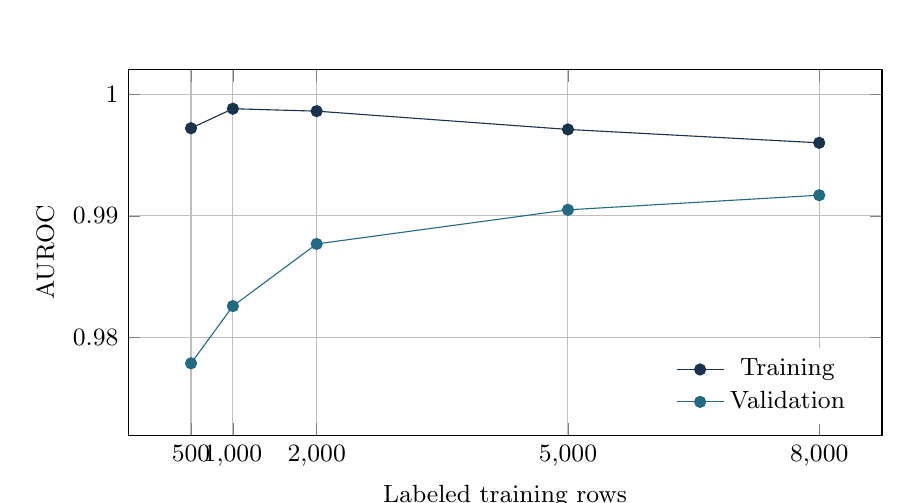
\begin{tikzpicture}
\begin{axis}[
  width=0.92\linewidth,
  height=2.45in,
  xlabel={Labeled training rows},
  ylabel={AUROC},
  xtick={500,1000,2000,5000,8000},
  ymin=0.972, ymax=1.002,
  legend pos=south east,
  grid=major,
  tick label style={font=\small},
  label style={font=\small},
  legend style={font=\small, draw=none},
]
\addplot[navy, mark=*] coordinates {(500,0.9972) (1000,0.9988) (2000,0.9986) (5000,0.9971) (8000,0.9960)};
\addlegendentry{Training}
\addplot[teal, mark=*] coordinates {(500,0.9779) (1000,0.9826) (2000,0.9877) (5000,0.9905) (8000,0.9917)};
\addlegendentry{Validation}
\end{axis}
\end{tikzpicture}
\end{center}

\smallnote{Same numbers as Q2.1. A PDF of this figure is also at \texttt{submissions/group-number-8/figures/learning\_curve.pdf}.}

\question{Q2.3 [3 points].}{What does the curve suggest about overfitting, underfitting, and the value of more labeled examples?}

The booster is not underfitting. Training AUROC stays above 0.996 at every size, and validation is already 0.9779 with 500 labeled rows, which is what we would expect if a few formatting rates carry most of the signal. The train--validation gap shrinks steadily, from 0.0193 at 500 rows to 0.0043 at 8{,}000, so the early gap is extra variance from a small sample rather than a model that cannot represent the holdout. Validation itself rises at every step: by 0.0047 from 500 to 1{,}000 rows, by 0.0051 from 1{,}000 to 2{,}000, by 0.0027 from 2{,}000 to 5{,}000, and by 0.0012 from 5{,}000 to 8{,}000. Past 2{,}000 labeled rows the gains are small. Training AUROC drifts down slightly over the same range (0.9988 at 1{,}000 rows, 0.9960 at 8{,}000) as the trees see a wider mix of pages and fit the training set a little less tightly. For this layout model, a few thousand labeled passages already capture nearly all of the in-collection gain.

\section{Learning from unlabeled data (5 points)}
\textbf{Learning goal:} test whether the additional 3,000 unlabeled passages help.
\question{Q3.1 [2 points].}{Describe one method that uses \texttt{unlabeled.csv} (e.g., self-training, confidence-based pseudo-labeling, clustering, or feature learning). How did you prevent validation-label leakage?}

We use the 3{,}000 unlabeled passages only as extra text for representation learning. The comparison model is the locked \texttt{sgd\_bpe} classifier. In the supervised run, BPE and TF-IDF are fit on the 8{,}000 labeled training rows. In the unlabeled run they are fit on those 8{,}000 rows plus the 3{,}000 unlabeled rows. No unlabeled label is invented, and the classifier is still fit only on the 8{,}000 labeled rows. Validation passages are in neither fit, and this comparison does not read \texttt{test.csv}. The BPE vocabulary stays at the cap of 30{,}000; the TF-IDF width goes from 389{,}838 columns to the 500{,}000-feature cap.

\question{Q3.2 [2 points].}{Compare against a supervised baseline under the same held-out validation protocol.}
\begin{tabularx}{\linewidth}{@{}Yp{1.5in}@{}}\toprule Method & Validation AUROC \\ \midrule
Supervised only (\texttt{sgd\_bpe}) & 0.9727 \\
BPE and TF-IDF also fit on \texttt{unlabeled.csv} & 0.9730 \\
\bottomrule\end{tabularx}

\question{Q3.3 [1 point].}{Did it help? Give a concrete, evidence-based explanation (including possible noise in pseudo-labels).}

It did not help in any way we would keep. The validation AUROC moves from 0.9727 to 0.9730, a change of $+0.0003$. That is smaller than the gap between neighboring SGD penalties in Q1.3 (0.0012 between $\alpha=5\cdot10^{-5}$ and $\alpha=10^{-4}$). There is no pseudo-label noise in this result, because we never assigned labels to the unlabeled rows. The likely reason the extra text does so little is that 8{,}000 passages already fill the 30{,}000 BPE merges, so the unlabeled rows mostly repeat subwords the vocabulary already has. They do change IDF enough to hit the feature cap, and that change does not move the holdout. We therefore leave unlabeled text out of the validation comparisons above. The Kaggle refit still fits BPE and TF-IDF on train, unlabeled, and test text, with classifiers trained only on labeled rows, matching the submission pipeline; that refit is not the comparison in this table.

\newpage
\section{Generalization and error analysis (20 points)}
\textbf{Learning goal:} characterize how well the selected model generalizes and where it fails. Use \textbf{labeled validation data}; hidden test labels and hidden domain/generator information are unavailable.

\question{Q4.1 [5 points].}{Compare training and validation AUROC for your final selected model. Is there a gap? What explanations are plausible?}

For \texttt{ENS\_top2} the training AUROC is 0.9999 and the validation AUROC is 0.9978, a gap of about 0.0021. The two members do not look the same. \texttt{sgd\_bpe} is 1.0000 on the training partition and 0.9727 on the holdout (gap about 0.027). \texttt{lr\_bpe} is the same shape (1.0000 and 0.9712). With 389{,}838 TF-IDF columns and 8{,}000 rows, a linear classifier can separate the training partition even when some of those directions are brittle. \texttt{gbm\_format} is 0.9960 against 0.9917, a gap of 0.0043, which matches a model with a few dozen shallow trees on 21 features. Rank averaging pulls the over-separated wording scores back toward the layout scores, and the ensemble gap ends up smaller than either wording model alone. A second reading of the small ensemble gap is less comforting: the holdout is a random slice of the same collection, so it does not contain the new domains or the edited AI passages described for the test set. A 0.002 gap here does not mean the submission will move by 0.002 on Kaggle.

\question{Q4.2 [5 points].}{Evaluate performance over at least three text-length bins (define the bins), or another observable subgroup available in your data. Explain why you chose the grouping.}
\begin{tabularx}{\linewidth}{@{}Yrr@{}}\toprule Subgroup / bin & Count & Validation AUROC \\ \midrule
Short, $\le 177$ words & 668 & 0.9972 \\
Medium, 178--241 words & 672 & 0.9985 \\
Long, $\ge 242$ words & 660 & 0.9984 \\
\bottomrule\end{tabularx}

Word count is observable without domain or generator labels, and the course data span roughly 75 to 350 words, so a length effect was a real possibility. The cut points are the tertiles of validation word count, 177 and 241, which put about a third of the holdout in each bin (mean lengths 142, 208, and 282 words). \texttt{ENS\_top2} is essentially flat across them: 0.9972, 0.9985, 0.9984. Length is not where this model fails inside the holdout. The errors in Q4.3 sit in every bin, from a 95-word review to recipes of about 300 words, and they line up with genre and formatting rather than with the tertile.

\question{Q4.3 [5 points].}{Analyze at least \textbf{five false positives and five false negatives} from your held-out validation set. Provide example IDs, predicted probabilities, and short failure hypotheses. Do not paste full passages unless essential.}
\begin{tabularx}{\linewidth}{@{}p{0.64in}p{0.70in}p{0.72in}Y@{}}\toprule ID & Error type & P(AI) & Possible reason \\ \midrule
961 & FP & 0.607 & Short movie review, one paragraph. Wording rank 0.59, layout rank 0.63. No blank line. \\
6378 & FP & 0.578 & Encyclopedia company lead. Wording rank 0.62 carries it; layout is 0.54. \\
9612 & FP & 0.572 & Encyclopedia paragraph on a research database. Wording rank 0.55, layout rank 0.60. \\
1181 & FP & 0.567 & Song article in the same register. Wording rank 0.62, layout 0.51. \\
4607 & FP & 0.563 & Informal forum question. Layout rank 0.51; wording rank 0.62. \\
5498 & FN & 0.323 & Lasagna recipe with hard newlines and no blank line. Layout rank 0.09; wording 0.55. \\
1602 & FN & 0.382 & Biography with a citation marker, no line breaks. Wording rank 0.32, layout 0.44. \\
7049 & FN & 0.414 & Bulleted ingredient list. Wording rank 0.32, layout 0.50. \\
2515 & FN & 0.422 & Line-broken tuna recipe. Wording rank 0.30, layout 0.54. \\
3401 & FN & 0.433 & First-person post that repeats one sentence. Wording rank 0.28, layout 0.59. \\
\bottomrule\end{tabularx}
\smallnote{False positive: human text with rank-average $\ge 0.5$. False negative: AI text with rank-average $< 0.5$. At this threshold the holdout has 29 false positives, 23 false negatives, and 1{,}948 correct rows. Member ranks are percentile ranks of the locked models on the validation set. The ten rows above are the highest-scoring false positives and the lowest-scoring false negatives.}

\question{Q4.4 [5 points].}{What recurring failure patterns did you identify, and how might you address one of them? Distinguish observed patterns from speculation.}

Two patterns are visible in the table, and one is visible in the training-partition feature means. First, all ten listed errors have no blank line. That is the layout cue with the largest class gap on the training partition (present in 0.4\% of human passages and 66.3\% of AI passages), so once it is absent the ensemble is scoring on weaker signals and the probabilities sit between 0.32 and 0.61. Second, the low false negatives are recipes or a repeated first-person post, and the high false positives are encyclopedia prose, a review, and a forum question. On the lasagna recipe the layout rank is 0.09 because the lines break like hard-wrapped human text. On the other recipes, the biography, and the repeated post, the wording rank is the one below 0.35: those n-grams look like ordinary web text, and a bag of 1--3 grams does not by itself record that one sentence was pasted many times.

We do not claim these ten rows are the test-set failure modes. It is a speculation, not a measurement, that blank lines will be edited away in the adversarial portion of the test set. What we can say from the holdout is that rank averaging cannot fix a row when both members land on the same side of one half. That is the biography, where both ranks are below 0.45, and it is the movie review and the database paragraph, where both ranks are above 0.54. The company lead and the song article are different: the layout rank is near 0.51--0.54 and the wording rank is about 0.62. One concrete next feature is a repetition rate, which would target the looped post without touching the layout cues. We did not add it in this submission.

\newpage
\section{Open-ended improvements and insights (15 points)}
\textbf{Learning goal:} propose and test one improvement beyond the required baseline comparisons. This can be simple: a targeted feature change, alternate regularization scheme, ensemble, different representation, augmentation, or training approach. Sophistication alone does not earn credit.

\question{Q5.1 [3 points].}{What specific question or hypothesis motivated your improvement? What weakness or opportunity did you observe?}

The layout booster was the best single model on the holdout (0.9917), and the wording models were close to each other and lower (0.9727 and 0.9712). The question was whether those two kinds of evidence make different mistakes. If they do, an average of their ranks should beat either one. A second question came immediately after: \texttt{lr\_bpe} and \texttt{sgd\_bpe} read the same TF-IDF matrix, so adding both of them to the average might only dilute the layout vote. We tested both averages on the same holdout, with every member's hyperparameters left at the locked values from Q1.3.

\question{Q5.2 [4 points].}{What exactly did you change? Describe the baseline, the new approach and what you held fixed for a fair comparison.}

The baseline is the locked \texttt{gbm\_format} model from Q1.2. The improvement, \texttt{ENS\_top2}, fits that booster and the locked \texttt{sgd\_bpe} model on the same 8{,}000 rows and replaces each decision score by its percentile rank inside the set being scored. The reported probability is the arithmetic mean of the two ranks. Ranks put a tree ensemble and a linear margin on one scale; AUROC depends only on order, so the monotone rescaling does not throw away a member's ranking. \texttt{ENS\_top3} does the same with \texttt{lr\_bpe} as a third rank. The validation ids, the BPE and TF-IDF fit (8{,}000 labeled rows only), and the classifier settings are unchanged. We did not refit the vectorizer on validation text, and we did not use test labels.

\question{Q5.3 [4 points].}{What were the measured results?}
\begin{tabularx}{\linewidth}{@{}YrrY@{}}\toprule Configuration & Val. AUROC & Runtime & Relevant difference \\ \midrule
\texttt{gbm\_format} & 0.9917 & 1.6 s & layout only \\
\texttt{ENS\_top2} & 0.9978 & 1.7 s & adds \texttt{sgd\_bpe}; Spearman with the booster is 0.725 \\
\texttt{ENS\_top3} & 0.9953 & 5.5 s & also adds \texttt{lr\_bpe}; that pair's Spearman is 0.988 \\
\bottomrule\end{tabularx}

\smallnote{Runtimes are the sum of member \texttt{fit} calls. The shared BPE and TF-IDF build (26.0 s) is extra for any row that uses wording features, and it is paid once. Mean predicted probability, instead of rank average, scores 0.9975 for \texttt{ENS\_top2} on the same holdout. We submit the rank average.}

\question{Q5.4 [4 points].}{What did you learn? Did the results support the hypothesis? What limits the conclusion, and what would you try next?}

The holdout supports both parts of the hypothesis. Combining the layout booster with the less correlated wording model raises validation AUROC from 0.9917 to 0.9978. Adding the second wording model, which correlates 0.988 with the first, lowers the average to 0.9953. Equal weights were enough; we did not need a learned stacking model to see the effect. The limit is the split. Both members were trained and scored on passages from one collection, and the layout features that make the booster strong are exactly the features a different export format would change. Q4.3 already shows the practical version of that limit: when the blank line is missing, the ensemble's probability falls back to a narrow band around one half, and a recipe with human-like line breaks is scored 0.32. The next experiment we would run, still on this same holdout, is a repetition feature aimed at looped generations, and a check of rows where the wording rank and the layout rank disagree by more than 0.3. We would not tune either idea on the Kaggle test labels.

\section{Code submission, reproducibility and AI assistance (10 points)}
\textbf{Submission format:} Submit a \textbf{GitHub PR URL} against the course repository. We will inspect the final code and its development history, not just the final snapshot. Do not squash away meaningful intermediate commits before review. Template \href{https://github.com/sekhari/human-or-ai-submissions}{here}.

\question{Q6.1 [5 points].}{Provide the PR URL, the entrypoint for training/evaluation, and the command used to generate \texttt{submission.csv}. State dependencies and random seeds.}

The PR is \url{https://github.com/sekhari/human-or-ai-submissions/pull/20}, from branch \texttt{Group-Number-8} of \url{https://github.com/CosineF/team8-human-or-ai-submissions}. Code lives in \texttt{submissions/group-number-8/}. Python 3.12, scikit-learn 1.5.2, \texttt{tokenizers} 0.20.3, and the other pins in \texttt{requirements.txt}. No pretrained language-model weights. Validation split seed 20261023. Classifier seed 42.

Report numbers, including the learning curve and this document's tables:

\begin{verbatim}
python train.py \
  --data-dir /path/to/cornell-tech-cs-5785-combined-2026-ai-vs-human-text \
  --mode report --seed 20261023
\end{verbatim}

That command writes \texttt{results/metrics.json} and \texttt{figures/learning\_curve.pdf}. It does not read \texttt{test.csv}.

Kaggle file (all 10{,}000 labels; BPE and TF-IDF see train, unlabeled, and test text; no test labels):

\begin{verbatim}
python train.py \
  --data-dir /path/to/cornell-tech-cs-5785-combined-2026-ai-vs-human-text \
  --mode submit --out submission.csv
\end{verbatim}

\texttt{submission.csv} is \texttt{ENS\_top2}. The same run also writes \texttt{submission\_ens\_top3.csv}, which we are not uploading, and \texttt{model.joblib}. Reloading that file reproduces the two-model CSV:

\begin{verbatim}
python predict.py --test /path/to/test.csv --model model.joblib --out submission.csv
\end{verbatim}

\question{Q6.2 [3 points].}{Give two or three examples of changes you made during development. Link to relevant commits or PR discussion and briefly explain what the experiments taught you.}

Three commits on branch \texttt{Group-Number-8} match the measurements above. First, \href{https://github.com/CosineF/team8-human-or-ai-submissions/commit/cd121343e80a7b5ebb6f3b1ef78d2142da0bc82e}{\texttt{cd12134}} compared the three single models on the fixed split. The layout booster led (validation 0.9917) and the two BPE linear models were near 0.97, with train AUROC 1. Second, \href{https://github.com/CosineF/team8-human-or-ai-submissions/commit/2d5217e84deb5d3ecfd19bc3f10e7f2fcabfe383}{\texttt{2d5217e}} added the learning curve, the unlabeled feature check, and the \texttt{gbm\_format} error analysis. That unlabeled fit moved \texttt{sgd\_bpe} only from 0.9727 to 0.9730, and we did not build a pseudo-labeling loop on top of it. Third, \href{https://github.com/CosineF/team8-human-or-ai-submissions/commit/d2999f96dfc1cec71d096be9914bc20ac2ce67cf}{\texttt{d2999f9}} added the rank averages. \texttt{ENS\_top2} reached 0.9978, and the Spearman correlation of 0.725 said the wording and layout scores were not copies of each other. \texttt{ENS\_top3} adds \texttt{lr\_bpe}, which correlates 0.988 with the SGD model, and the three-model average fell to 0.9953, so the file we upload stayed the two-model average.

\question{Q6.3 [2 points].}{How did you use AI tools (such as Claude, ChatGPT or Copilot) for code, debugging, analysis or writing? What did you verify or modify yourself?}

An AI coding assistant helped turn the model definitions into \texttt{train.py} and \texttt{predict.py}, and it drafted sentences in this report from \texttt{results/metrics.json}. We read those answers together in person. We chose the five models, the rank average, and the decision to upload \texttt{ENS\_top2}. Every AUROC, count, and error id in the tables was produced by \texttt{python train.py --mode report} with seed 20261023, and we checked the split (2{,}000 rows, 1{,}000/1{,}000, no id overlap, no identical text) before using the file. The assistant did not label test passages, and we did not pull labels from an outside source. The Kaggle public score 0.95611 is the score shown for the uploaded \texttt{submission.csv}.

\textbf{AI policy.} You may use AI assistants for coding, debugging, explanations, brainstorming, and editing. We expect each team to exercise its own judgment, run experiments, check outputs, and understand its submitted approach. Sending the entire assignment to an AI tool and submitting its unverified output without meaningful involvement does not satisfy the objectives of this project. We will use the PR history, reproducible experiments and report together as evidence of engagement. \emph{Commit counts and the presence of AI-generated code are not themselves grading criteria.} Do not fabricate results or retrieve hidden test labels.


\section*{Final submission checklist}
\begin{itemize}[label=$\square$]
\item Final probabilities submitted to Kaggle for every \texttt{test.csv} ID.
\item Completed report, with all required answers, tables, figures and sources, submitted as PDF.
\item GitHub PR linked on the report title page and in the course submission portal.
\item Code and dependencies recreate final predictions (within reasonable numerical tolerance).
\item Relevant experiments and seed/configuration details are recorded.
\item AI-use disclosure is complete; hidden labels were not retrieved externally.
\end{itemize}


\end{document}
